\chapter{\label{ch:archetype modal}Modal Example}

\section{\label{sec:modal problem}Modal Approximation}  %    S    S    S    S    S    S    S    S    S
The following example represents a problem in linear regression. A sequence of $m$ data points $\paren{x_{k}, T_{k}}$, $k=1\colon m$ are recored. The goal is to find the best approximation to a straight line. The \emph{trial function} is
  \begin{equation*}   %  =   =   =   =   =
    y(x) = a_{0} + a_{1} x .
    \label{eq:lr trial}
  \end{equation*}
The residual errors are the difference between the measurements and predictions:\\
\begin{center}
residual error$_{k}$ = measurement$_{k}$ -- prediction$_{k}$.
\end{center} 
 More formally the residual error is
  \begin{equation*}   %  =   =   =   =   =
  %\begin{split}
    r_{k} = T_{k} - y(x_{k}), \quad k=1\colon m.
    %\label{eq:}
  %\end{split}
  \end{equation*}
From this springs the \emph{merit function}, the target of minimization,
  \begin{equation}   %  =   =   =   =   =
  \begin{split}
    M(a) 
      &= \sum_{k=1}^{m} r_{k}^{2} \\
      &= \sum_{k=1}^{m} \paren{\text{measurement}_{k} - \text{prediction}_{k}}^{2} \\
      &= \sum_{k=1}^{m} \paren{T_{k} - y\paren{x_{k}}}^{2} \\
      &= \sum_{k=1}^{m} \paren{T_{k} - a_{0} - a_{1} x_{k}}^{2}
    \label{eqn:merit}
  \end{split}
  \end{equation}
The least squares solution $a_{LS}$ is formally defined as 
  \begin{equation*}   %  =   =   =   =   =
  %\begin{split}
    a_{LS} = \lst{a \in \cmplx{2} \colon \normts{y(x_{k}) - a_{0} - a_{1} x_{k}} \text{ is minimized} }.
    %\label{eq:}
  %\end{split}
  \end{equation*}
The solution satisfies
  \begin{equation}   %  =   =   =   =   =
  %\begin{split}
    \nabla M( a )|_{a_{LS}} = 0 .
    \label{eq:gradient lr}
  %\end{split}
  \end{equation}

\section{\label{sec:bevington example}Bevington Example}  %    S    S    S    S    S    S    S    S    S
\subsection{Problem Statement}  %   SS   SS   SS   SS   SS   SS   SS   SS   SS   SS   SS   SS
To provide a common reference, see the example in \cite[ch 6]{Bevington}. The data is summarized below in table \ref{tab:bevington data and results}. The problem involves temperature measurements $T_{k}$ made at position $x_{k}$. 

\begin{table}[h]
	\begin{center}
		\begin{tabular}{rcc|rr@{.}l}
		  %
		  & \multicolumn{2}{c}{Input} &  \multicolumn{3}{c}{Output} \\
		  %
		  $k$ & $x_{k} (cm) $ & $T_{k} (^{\circ}C)$ & $y\paren{x_{k}} (^{\circ}C)$ & \multicolumn{2}{c}{$r_{k} (^{\circ}C)$} \\\hline
		  %
			 1 & 1 & 15.6 & 14.2222 & --1 & 37778 \\
			 2 & 2 & 17.5 & 23.6306 &   6 & 13056 \\
			 3 & 3 & 36.6 & 33.0389 & --3 & 56111 \\
			 4 & 4 & 43.8 & 42.4472 & --1 & 35278 \\
			 5 & 5 & 58.2 & 51.8556 & --6 & 34444 \\
			 6 & 6 & 61.6 & 61.2639 & --0 & 336111 \\
			 7 & 7 & 64.2 & 70.6722 &   6 & 47222 \\
			 8 & 8 & 70.4 & 80.0806 &   9 & 68056 \\
			 9 & 9 & 98.8 & 89.4889 & --9 & 31111 \\
		  %
		\end{tabular}
	\end{center}
	\caption{Raw data and results.}
	\label{tab:bevington data and results}
\end{table}%

\begin{figure}[htbp] %  figure placement: here, top, bottom, or page
   \centering
   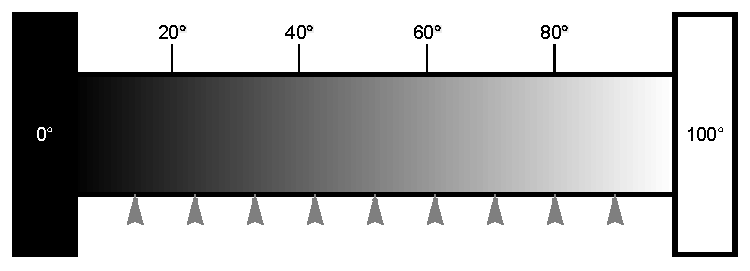
\includegraphics[ width = 3in ]{\pathgraphics "bevington classic"/bar} 
   \caption[Measuring the temperature of a bar.]{Measuring the temperature of a bar held between two constant-temperature heat baths.}
   \label{fig:bar}
\end{figure}

  \begin{table}[htbp]  %  T A B L E
    \caption{Problem statement for linear regression.}
    \begin{center}
      \begin{tabular}{lll}
        %
        \bf{trial function} & $T(x) = a_{0} + a_{1} x$ \\
        \bf{merit function} & $M(a) = \sum_{k=1}^{m}\paren{T_{k} - a_{0} - a_{1} x}^{2}$ \\
        \bf{measurements}   & $x_{k}$, $k=1\colon m$ & position, cm \\
                            & $T_{k}$, $k=1\colon m$ & temperature, $^{\circ} C$ \\
        \bf{results}        & $a_{0} \pm \eps_{0}$, $^{\circ}$C & intercept \\
                            & $a_{1} \pm \eps_{1}$, $^{\circ}$C / cm & slope \\
        \bf{residual error} & $r_{k} = T_{k} - a_{0} - a_{1} x$, $^{\circ} C$ \\
        \bf{linear system}  & $\mat{cc}{1 & x_{1}  \\ \vdots & \vdots \\ 1 & x_{m}} 
                               \mat{c}{a_{0} \\ a_{1}} = 
                               \mat{c}{T_{1} \\ \vdots \\ T_{m}}$ \\
        \bf{ideal solution} & $\mat{c}{a_{0}\\a_{1}} = \mat{c}{0\\1}$ \\
        %
      \end{tabular}
    \end{center}
  %\label{tab:?}
  \end{table}%

\subsection{\label{ssec:Normal Equations via Calculus}Normal Equations via Calculus}  %   SS   SS   SS   SS   SS   SS   SS   SS   SS   SS   SS   SS
In \S 6.4, Bevington solves the problem by applying calculus to the final form in \eqref{eqn:merit}, effectively solving \eqref{eq:gradient lr}. Introducing the notation
  \begin{equation*}   %  =   =   =   =   =
  %\begin{split}
       \partial_{j} M = \frac{\partial M(a_{0}, a_{1})}{\partial a_{j}}
    %\label{eq:}
  %\end{split}
  \end{equation*}
the simultaneous equations to solve are
\begin{equation*}
  \begin{split}
    &-2 \sum_{k} \paren{T_{k} - a_{0} - a_{1}x_{k}} \phantom{x_{k}} = 0, \\
    &-2 \sum_{k} \paren{T_{k} - a_{0} - a_{1}x_{k}} x_{k}  = 0.
  \end{split}
\end{equation*}
Rewriting in a more revealing form \\
  %
  \begin{table}[h!]  %  T A B L E
    %\caption{default}
    \begin{center}
      \begin{tabular}{lclcl}
        %
         $\sum T_{k}$     & = & $a_{0} \sum 1$     & $ + $ & $a_{1} \sum x_{k}$, \\
         $\sum T_{k} x_{k}$ & = & $a_{0} \sum x_{k}$ & $ + $ & $a_{1} \sum x_{k}^{2}$. \\
        %
      \end{tabular}
    \end{center}
  %\label{tab:?}
  \end{table} \\
  %
Recast as a linear system, the minimization criteria become
  \begin{equation}   %  =   =   =   =   =
      \mat{ll}{\sum 1 & \sum x_{k} \\ \sum x_{k} & \sum x_{k}^{2}}
      \mat{c}{a_{0} \\ a_{1} } = 
      \mat{l}{\sum T_{k} \\ \sum x_{k}T_{k}}
    \label{eq:modal matrix eq}
  \end{equation}
where summation from 1 to $m$ is implied. (Therefore $\sum 1 = m$.)

Defining the determinant
  \begin{equation*}   %  =   =   =   =   =
  %\begin{split}
    \Delta = m \sum x_{k}^{2} - \paren{\sum x_{k}}^{2}
    %\label{eq:}
  %\end{split}
  \end{equation*}
the matrix inverse is
  \begin{equation*}   %  =   =   =   =   =
  %\begin{split}
    \mat{cl}{m & \sum x_{k} \\ \sum x_{k} & \sum x_{k}^{2}}^{-1} = \Delta^{-1} 
    \mat{lc}{\ps \sum x_{k}^{2} & -\sum x_{k} \\ -\sum x_{k} & m }
    %\label{eq:}
  %\end{split}
  \end{equation*}
The solution to equation \eqref{eq:modal matrix eq} is the matrix product
  % = =  e q u a t i o n
  \begin{equation*}
    \mat{c}{a_{0} \\ a_{1} } = \Delta^{-1}
    \mat{ll}{\ps \sum x_{k}^{2} & -\sum x_{k} \\ -\sum x_{k} & \ps \sum 1}
    \mat{l}{\sum T_{k} \\ \sum T_{k} x_{k}}
    \label{eqn:bevington solution product}
  \end{equation*}
  % = =
Compare the final results to Bevington's equations 6-19:
  \begin{equation*}
  \begin{split}
    a_{0} &= \Delta^{-1} \paren{\sum x_{k}^{2}\sum T_{k} - \sum x_{k}\sum x_{k}T_{k}}, \\
    a_{1} &= \Delta^{-1} \paren{m \sum x_{k}T_{k} - \sum x_{k}\sum T_{k}}.
  \label{eqn:bevington soln}
  \end{split}
  \end{equation*}
  
\section{\label{sec:bevington example}Bevington Solution}  %    S    S    S    S    S    S    S    S    S

\subsection{Fit Parameters}  %   SS   SS   SS   SS   SS   SS   SS   SS   SS   SS   SS   SS
  \begin{equation*}   %  =   =   =   =   =
  %\begin{split}
      a = \mat{c}{a_{0} \\ a_{1}} = \frac{1}{360} \mat{c}{1733 \\ 3387}
    %\label{eq:}
  %\end{split}
  \end{equation*}

\subsection{Error Propagation}  %   SS   SS   SS   SS   SS   SS   SS   SS   SS   SS   SS   SS

Bevington's greatest contribution may be his masterful explanation of error propagation.
% = =  e q u a t i o n
  \begin{equation*}
    %\begin{split}
    s^{2} \approx \frac{\rtr{T}} {m-n}
    %\end{split}
    %\label{eqn:}
  \end{equation*}
% = =
\begin{equation*}
  \begin{split}
    %
    \eps_{0}^{2} &= \frac{r^{\mathrm{T}}r}{\Delta\paren{m-n}} \sum x_{k}^{2} \\
    \eps_{1}^{2} &= \frac{r^{\mathrm{T}}r}{\Delta\paren{m-n}} \sum 1 \\
    %
  \end{split}
  \label{eqn:bevington error terms}
\end{equation*}

The residual error vector is
% = =  e q u a t i o n
  \begin{equation*}
    %\begin{split}
      r = \frac{1}{360}
          \mat{r}{-496 \\ 2207 \\ -1282 \\ -487 \\ -2284 \\ -121 \\ 2330 \\ 3485 \\ -3352}
    %\end{split}
    %\label{eqn:}
  \end{equation*}
% = =
making the total error
% = =  e q u a t i o n
  \begin{equation*}
    %\begin{split}
      \rtr{T} = \frac{1\,139\,969}{3600}
    %\end{split}
    %\label{eqn:}
  \end{equation*}
% = =

  \begin{equation*}   %  =   =   =   =   =
  %\begin{split}
    \Delta = 540
    %\label{eq:}
  %\end{split}
  \end{equation*}
  \begin{equation*}   %  =   =   =   =   =
  %\begin{split}
    \eps = \mat{c}{\eps_{0} \\ \eps_{1}} = 
    \paren{360\sqrt{35}}^{-1}
    \sqrt{ \mat{r}{108\,297\,055 \\ 3\,419\,907} }
    %\label{eq:}
  %\end{split}
  \end{equation*}
\subsection{Final Answer}  %   SS   SS   SS   SS   SS   SS   SS   SS   SS   SS   SS   SS

The results in equation \eqref{eqn:soln vector}.
% = =  e q u a t i o n
  \begin{equation*}
    \begin{split}
      a_{0} &= 4.8 \pm 4.9 \quad \text{\ \ \ (intercept)} \\
      a_{1} &= 9.41 \pm 0.87 \quad \text{(slope)}
    \end{split}
    \label{eqn:soln vector}
  \end{equation*}
% = =
An alternative presentation is
% = =  e q u a t i o n
  \begin{equation*}
    \begin{split}
      a_{0} &= 4.8 \paren{4.9} \quad \text{\ \ \ (intercept)} \\
      a_{1} &= 9.41 \paren{0.87} \quad \text{(slope)}
    \end{split}
    %\label{eqn:}
  \end{equation*}
% = =

\section{Vizualization}  %    S    S    S    S    S    S    S    S    S

\subsection{Seeing the Solution}  %   SS   SS   SS   SS   SS   SS   SS   SS   SS   SS   SS   SS

\begin{figure}[htbp] %  figure placement: here, top, bottom, or page
   \centering
   \includegraphics[ width = 4.0in ]{\pathgraphics "bevington classic"/"red bars"} 
   \caption[Solution plotted against data with residual errors shown in red.]{Solution plotted against data with residual errors shown in red.}
   %\label{fig:example}
\end{figure}

\begin{figure}[htbp] %  figure placement: here, top, bottom, or page
   \centering
   \includegraphics[ width = 4.0in ]{\pathgraphics "bevington classic"/"residuals"} 
   \caption[Scatter plot of residual errors.]{Scatter plot of residual errors.}
   %\label{fig:example}
\end{figure}

\subsection{Digger Deeper}  %   SS   SS   SS   SS   SS   SS   SS   SS   SS   SS   SS   SS


\begin{figure}[htbp] %  figure placement: here, top, bottom, or page
   \centering
   \includegraphics[ width = 4.0in ]{\pathgraphics "bevington plus"/"merit bullseye"} 
   \caption[The merit function.]{The merit function in \eqref{eqn:merit} showing the solution (white cross) and three error bands in yellow.}
   %\label{fig:example}
\end{figure}

\begin{figure}[htbp] %  figure placement: here, top, bottom, or page
   \centering
   \includegraphics[ width = 4.0in ]{\pathgraphics "bevington plus"/"merit fancy"} 
   \caption[Another look at the merit function.]{Another look at the merit function in  \eqref{eqn:merit} showing the uncertainty parameters as elliptic radii.}
   %\label{fig:example}
\end{figure}

\begin{figure}[htbp] %  figure placement: here, top, bottom, or page
   \centering
   \includegraphics[ width = 3in ]{\pathgraphics "bevington plus"/"needle intercept"} \\[30pt]
   \includegraphics[ width = 3in ]{\pathgraphics "bevington plus"/"needle slope"}
   \caption{Solutions as normal distributions.}
   %\label{fig:example}
\end{figure}

\begin{figure}[htbp] %  figure placement: here, top, bottom, or page
   \centering
   \includegraphics[ width = 3.5in ]{\pathgraphics "bevington plus"/"whiskers"} 
   \caption[Whisker plot.]{Whisker plot.}
   %\label{fig:example}
\end{figure}

\endinput